\chapter{模式与出发时间选择方法的训练与评估}

建立好深度强化学习模型后,进行训练和评价对模型的发展和应用具有重大意义。这一过程可以从多方面优化模型性能,为模型在实际应用中的选用提供依据。首先,训练和评价过程可以验证模型的有效性,确保模型能够有效解决所面临的问题。训练过程使智能体学会最优策略,而评价过程则有助于了解模型在实际应用场景中的性能表现。其次,训练和评价过程有助于提高模型性能。智能体在训练过程中持续优化神经网络参数,提高任务表现。评价过程揭示了模型在某些方面的不足,为进一步优化提供线索。训练和评价过程还可以揭示不同算法在特定任务上的优劣,为实际应用中的算法选择提供依据。同时,对现有模型的训练和评价可以发现算法存在的问题和不足,激发新的算法研究和改进,进而推动深度强化学习领域的发展。总之,建立好模型后的训练和评价过程不仅能全面了解模型性能表现,提高泛化能力,优化参数设置,还能为算法选择和领域研究提供重要支持。


在本章中,将对上一章中提出的基于深度强化学习的出行模式与时间选择模型进行训练,并对训练结果进行详细分析,以了解模型的收敛速度和稳定性。此外,本章还将对模型进行评估,包括与传统方法的对比和模型参数的灵敏性分析,以验证模型的有效性。


\section{模型的训练与分析}

在本节中,将对上一章提出的算法模型进行训练,并对训练结果进行详细分析。通过观察训练过程中的学习曲线和计算累积奖励,可以深入了解模型在训练过程中的性能变化和整体表现。学习曲线和累积奖励作为评估深度强化学习模型表现的关键指标,能够从多方面反映模型性能。学习曲线揭示了模型在训练过程中的性能变化,有助于判断模型收敛速度和稳定性;累积奖励则反映智能体在任务中的整体表现,可以用于比较不同模型或算法的相对性能优劣。此外,这些指标还有助于评估模型的泛化能力和算法效率。观察学习曲线和累积奖励在训练集与测试集上的表现,可以判断模型是否适应新环境;同时,学习曲线还能反映算法在训练过程中的效率差异。因此,这些指标为模型优化、算法选择和参数调整提供了重要依据。

\subsection{实验场景的设置}

在训练之前,先确定一系列仿真参数来构建训练模型的场景。表\ref{public}列出了数值实验中使用的各个参数及其描述和取值。这些参数反映了不同出行方式的特点,如公交车和地铁的票价、运行频率和停留时间等。此外,还包括了如时间价值、提前到达和迟到的时间表延误成本等与个体出行决策相关的因素。
\renewcommand{\arraystretch}{1.2}
\setlength{\tabcolsep}{8mm}
\begin{table}[htbp]
\centering
\caption{实验中使用的仿真参数取值}
\label{public}
\begin{tabular}{lcl}
\toprule
参数 & 描述                                                 & 数值 \\ 
\midrule
$t_\text{min}$  & 最早出发时间                                     & 07:00 \\
$t_\text{max}$  & 最晚出发时间                                     & 09:00 \\
$t_\text{unit}$  & 出发时间选择的单位间隔(分钟)                   & 30    \\
$E_1$  & 将成本映射到奖励的常数                               & 100   \\
$E_2$  & 将成本映射到奖励的常数                               & 0.1   \\
$\alpha$  & 时间价值(元/分钟)                               & 0.5   \\
$\beta$  & 提前到达的时间表延误的单位成本(元/分钟)           & 0.05  \\
$\gamma$  & 迟到的时间表延误的单位成本(元/分钟)             & 0.3   \\
$o$  & 燃油价格(元/公里)                                 & 0.56  \\
\textbackslash{}  & 公交票价(元)                             & 2     \\
\textbackslash{}  & 地铁起步票价(元)                         & 1     \\
\textbackslash{}  & 地铁每公里递增票价(元/公里)               & 0.2   \\
\textbackslash{}  & 公交高峰频率(辆/小时)                      & 10    \\
\textbackslash{}  & 地铁高峰频率(辆/小时)                      & 14    \\
\textbackslash{}  & 公交非高峰频率(辆/小时)                    & 6     \\
\textbackslash{}  & 地铁非高峰频率(辆/小时)                    & 8     \\
\textbackslash{}  & 公交停留时间(秒)                           & 40    \\
\textbackslash{}  & 地铁停留时间(秒)                           & 30    \\ 
\bottomrule
\end{tabular}
\end{table}



\subsection{智能体的聚类与选取}


选择60个具有时间依赖性的起点-终点(OD)出行旅程作为智能体选取的样本集,并将它们的旅行特征输入到聚类方法中。表\ref{tab:sample_all}为部分出行的相关信息,包含出行ID,出发时间,出发路段,到达路段,与公共交通的可达性。

\renewcommand{\arraystretch}{1.2}
\begin{table}[htbp]
\centering
\caption{智能体部分样本数据示例}
\label{tab:sample_all}

\begin{adjustbox}{center}
\resizebox{\textwidth}{!}{
\begin{tabular}{cccccc}
\toprule
出行ID & 出发时间[s]  &    出发路段         &到达路段 &行程距离[km]   & 可达性[km] \\ 
\midrule
1	& 76	& 912\@941\#0 &	922\@772\#0 &	6.37&	1.48 \\
2	& 267 &	109\@758\#0 & 	673\@925\#0 &	2.89&	0.89 \\
3	& 331 &	76\@760\#0&	98\@918\#0&	5.56&	1.89\\
4&	0&	818\@890\#0&	27\@601\#0	&4.21	&1.93   \\
...&	...&	...&	...&...	&...   \\
60&	18&	818\@890\#0&	819\@24\#0&	3.41&	0.32  \\
\bottomrule
\end{tabular}}
\end{adjustbox}
\end{table}


在实施DBSCAN算法的过程中,需要确定两个关键参数:邻域半径($\mu$)和最小样本数($m$)。邻域半径的选取至关重要,因为它决定了算法认定哪些点属于同一个簇。如果两个点之间的距离小于邻域半径,那么就认为这两个点属于同一个簇。另一个关键参数是最小样本数,它表示一个簇中至少需要包含$m$个样本才能被认定为有效簇。这两个参数的选择会直接影响到聚类结果的质量,因此需要慎重考虑。

在本研究中,选择了经验法来确定DBSCAN算法的参数。经验法是一种依赖于经验或常识的方法,通过手动调整邻域半径和最小样本数的值来寻找最佳参数组合。首先尝试了不同的邻域半径和最小样本数组合,同时记录每种组合的轮廓系数得分。轮廓系数是一种用于评估聚类结果质量的指标,其值介于$-1$和$1$之间。计算轮廓系数的方法是将一个样本的簇内平均距离($a$)与与其最近簇的所有样本的簇内平均距离($b$)进行比较,计算得出该样本的轮廓系数为${(b-a)} / {max(a,b)}$,然后计算所有样本的轮廓系数的平均值。轮廓系数越接近1,说明聚类效果越好;越接近-1,说明聚类效果较差。

为了展示这一过程,表\ref{tab_cluster}呈现了尝试过的不同参数组合及其对应的轮廓系数得分。这有助于选择出最佳参数组合,从而提高聚类结果的质量。通过这种方法,可以确保在处理具有代表性的个体时,采用了较为合适的聚类参数。

\renewcommand{\arraystretch}{1.2} % 使表格行间距加大1.5倍
\setlength{\tabcolsep}{8mm}
\begin{table}[htbp]
\centering
\caption{参数组合及轮廓系数得分表}
\label{tab_cluster}
\begin{tabular}{ccc}
\toprule
邻域半径 ($\mu$) & 最小样本数 ($m$) & 轮廓系数得分       \\
\midrule
0.3 & 2 & 0.75 \\ 
0.3 & 3 & 0.72 \\ 
0.5 & 2 & 0.82 \\ 
0.5 & 3 & 0.79 \\ 
0.7 & 2 & 0.76 \\ 
0.7 & 3 & 0.74 \\ 

\bottomrule
\end{tabular}
\end{table}

通过实验,发现最佳参数组合为邻域半径为0.5,最小样本数为2。在这个参数组合下,得到的轮廓系数为0.82,表明聚类效果良好。将最小点数设置为10和最小距离阈值设置为0.05,共得到了4个类别以及2个噪声点,聚类的结果如图\ref{db_cluster}所示,图中标识的4个代表点将作为代表智能体,在训练时其经验被放入公共记忆池中。
\begin{figure}[H]
  \centering
  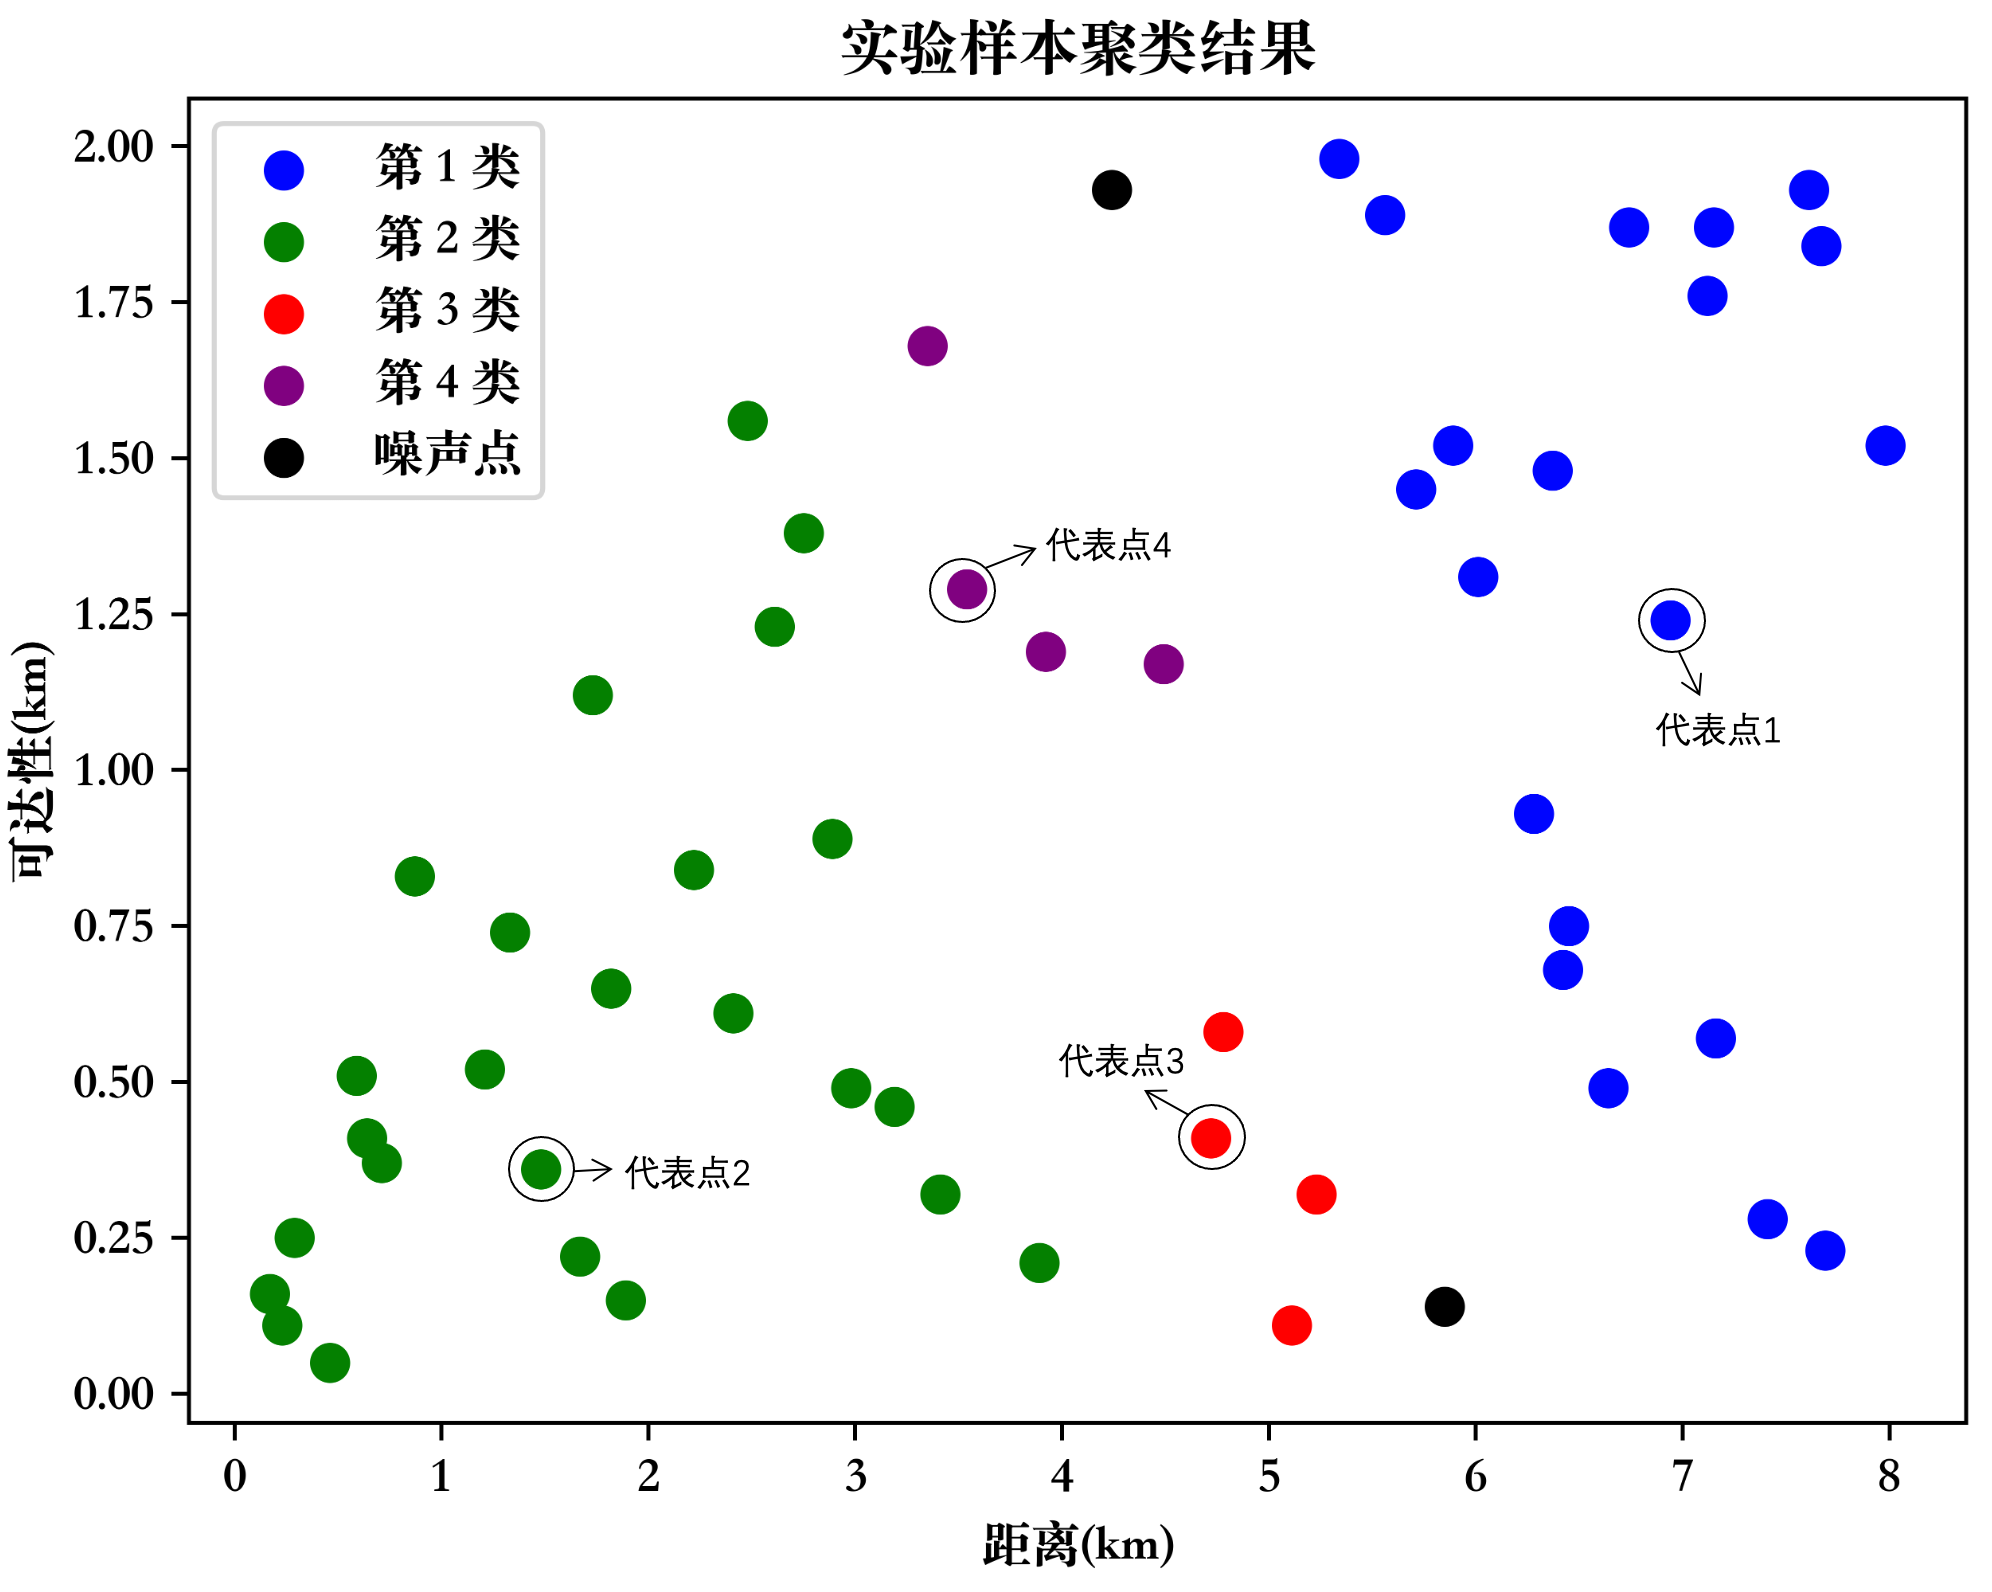
\includegraphics[width=.75\linewidth]{figures/content/db_cluster.png}
  \caption{代表智能体的位置示意图}
  \label{db_cluster}
\end{figure}


\subsection{训练以及结果分析}

在本文中,采用深度Q网络算法来优化出行模式和出发时间的选择,以获得最佳的出行体验。有数值实验均在标准计算机上进行,配置为Intel Core (TM) i5-9400F 2.90 GHz CPU和8 GB RAM。将训练过程设置为800个episode。在每个时间步长内,智能体根据当前状态选择一个动作,然后接收到环境返回的奖励,并转移到下一个状态。我们使用$\varepsilon$-贪婪策略来探索动作空间,其中$\varepsilon$在前400个episode中线性下降到0.1,然后保持不变。在探索时,智能体将以$\varepsilon$的概率选择一个随机动作,否则将根据当前Q值估计选择一个最佳动作。

所有数值实验的结果都是通过该算法的执行而得出的。使用SUMO仿真工具来模拟城市交通网络,四个代表智能体的OD在网络中的位置如图\ref{agent_map}所示,将智能体的行为应用于仿真中的出行模式选择和出发时间选择中。根据仿真结果,我们可以获得出行时间、路线和交通方式等方面的信息,以评估该算法的性能。
\begin{figure}
  \centering
  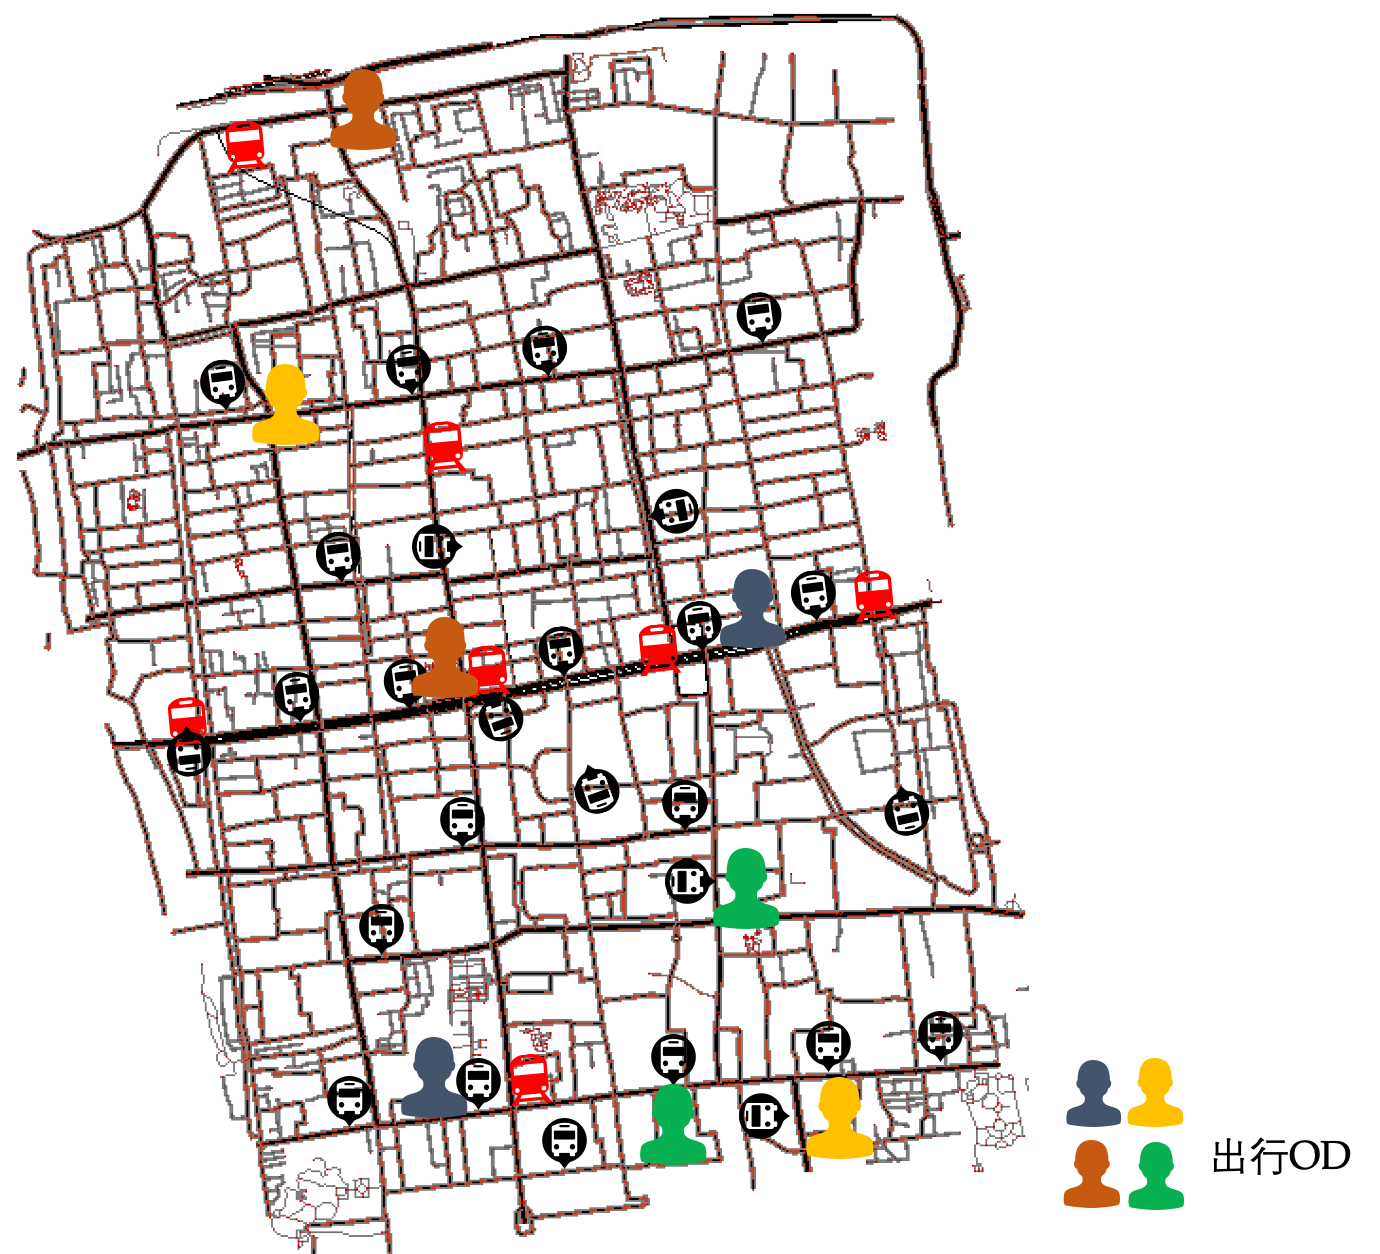
\includegraphics[width=.75\linewidth]{figures/content/agent_map.png}
  \caption{代表智能体的位置示意图}
  \label{agent_map}
\end{figure}

首先,在训练过程中设置了一个经验回放机制。该机制用于存储代理在仿真环境中所经历的状态、动作、奖励和下一状态等信息,并且按照一定的概率进行抽样,以保证数据的独立性和随机性。其次,采用目标网络的方法来减小估计误差的影响。在训练过程中使用了两个神经网络,即一个本地网络和一个目标网络。本地网络用于根据当前状态计算Q值,而目标网络则用于计算目标Q值。在一定的时间间隔内,目标网络的参数会从本地网络中更新,以缓解估计误差的影响。最后,将使用Adam优化器来对网络进行训练,以提高算法的收敛速度和性能。

图\ref{combine}显示了训练800个周期后,损失函数收敛模式的变化情况。整体下降趋势是明显的,是期望的。在早期阶段,损失函数值存在显著波动,这是由于行动探索以及代理在开始时对环境一无所知所致。然而,这种波动主要持续在前300个周期内,并且持续时间不长。实际上,从大约500个周期开始,损失函数值显示出最小的变化,几乎落在一条直线上。这种观察明确表明了算法的收敛性。可以看出,DQN算法在训练时获得了很好的表现,并且在这个任务上已经收敛。对于此任务的最终结果,我们可以通过计算平均旅行时间和平均出行成本来评估算法的性能。

在训练过程中,我们还对模型的参数进行了敏感性分析。我们主要考虑了两个参数:折现因子和经验回放缓冲区大小。折现因子决定了智能体对未来奖励的重视程度,而经验回放缓冲区大小则决定了模型从中学习的数据量。我们分别将折现因子设置为0.7和0.9,并将经验回放缓冲区大小设置为10000和50000。实验结果表明,当折现因子为0.9时,算法性能更好。而经验回放缓冲区的大小对算法性能的影响相对较小,但是当其增大到50000时,算法的性能有所提高。

综上所述,本文提出了一种基于DQN的多模式出行方式和出发时间选择方法。该方法不仅可以获得高效和准确的交通出行方式和出发时间选择策略,而且可以适应不同的交通模式和出行需求。通过在SUMO仿真环境中进行数值实验,我们验证了该方法的有效性和可行性。未来的研究方向可以包括进一步探索奖励函数设计、模型参数调整和增加更多交通模式的应用等。

在模型评估方面,我们首先评估了训练过程中每个代表性个体接收到的奖励变化情况。如图所示,我们检查了每个代表个体在训练过程中遵循DRL建议的行动所获得的奖励变化。考虑到每个代表个体的旅行都具有不同的时间依赖的OD点,因此相关的奖励处于不同的数量级。可以清楚地看出,代表者可能具有最长的旅程,而代表者3和4可能具有较短的旅程。尽管奖励的绝对值不同,但所有代表个体的曲线均呈递增趋势,这意味着他们通过与环境的交互和学习不断改进他们的旅行选择。在大约700次迭代之内,每个代表的奖励基本上稳定,此后变化不大,这一观察结果与图中的结果相符。

在图\ref{agents}中,我们图形化展示了四个代表性个体在训练过程中遵循的DRL建议行动。可以立即看出,在训练的开始阶段,代表者的行动经常变化,这是行动探索阶段。但是,一旦进入行动利用阶段,我们不再看到这种波动性,每个代表个体似乎已经找到了其自身JTMDTC问题的最优解。利用阶段期间的偶尔行动更改很可能是由于$\varepsilon$-贪心策略(其中$\varepsilon$已减小到非常小的值)触发的随机行动选择的结果。


\begin{figure}[htbp]
  \centering
  \subfloat[Representative \#1]{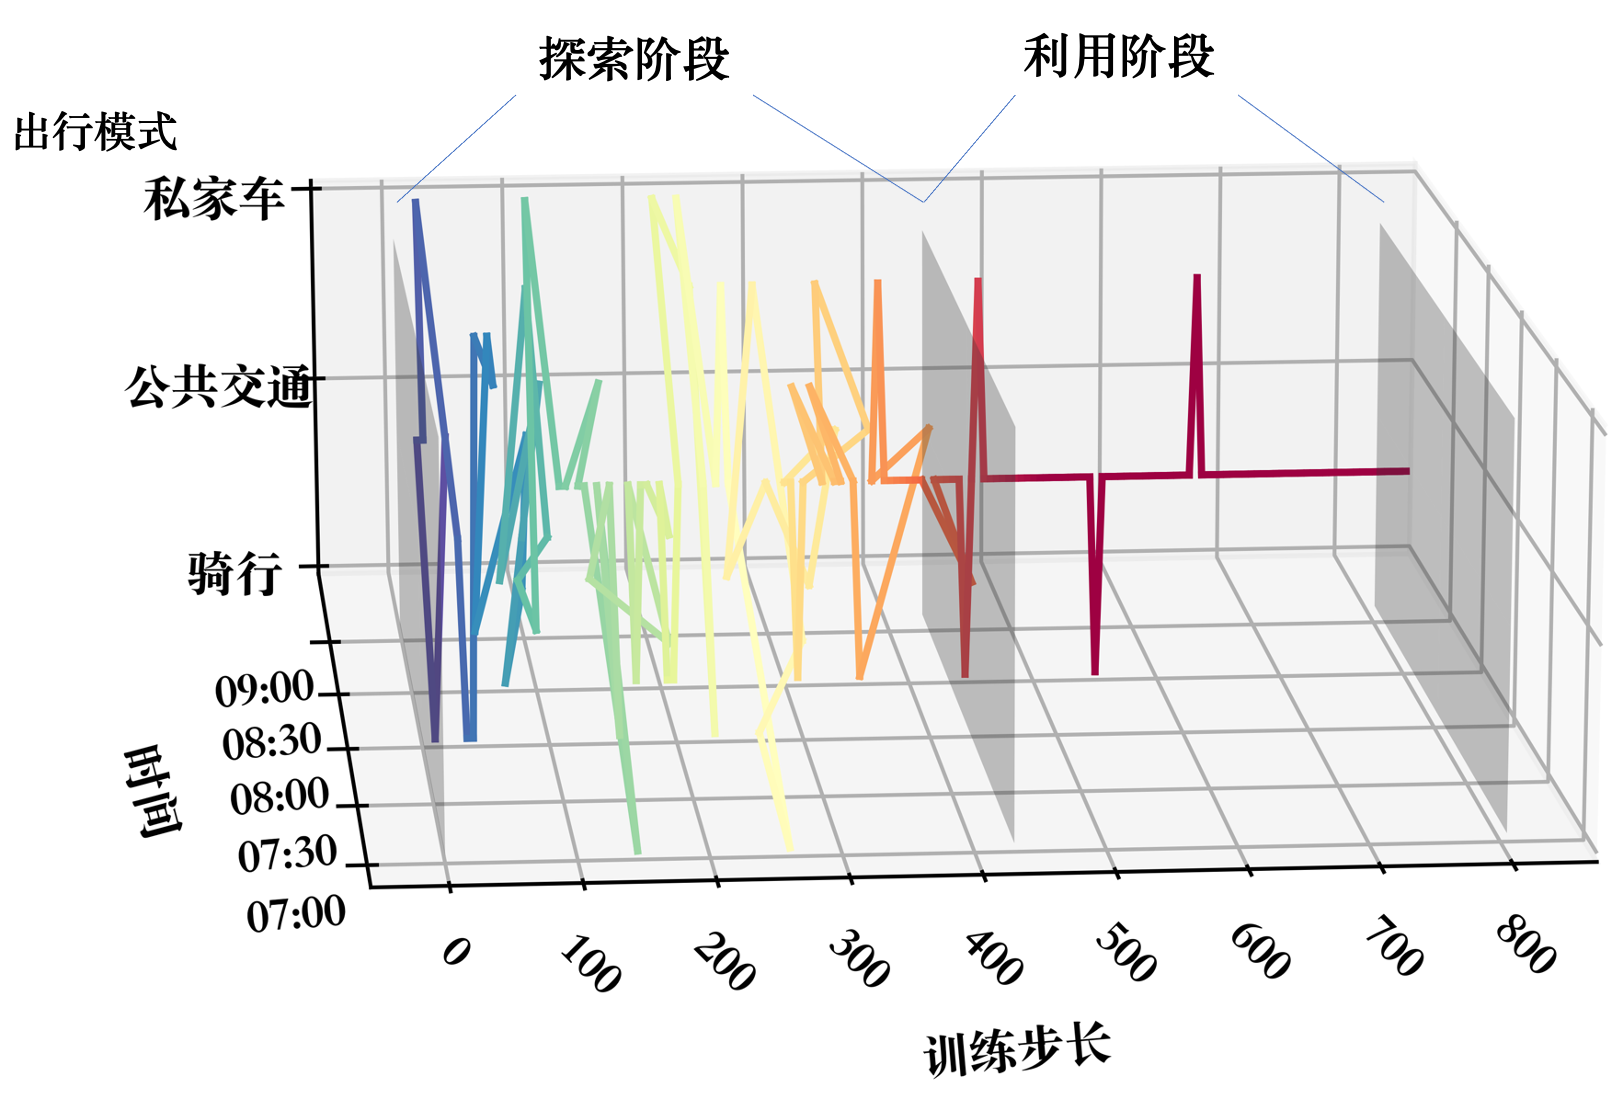
\includegraphics[width=.5\textwidth]{figures/content/action1.png}}
  \quad\quad
  \subfloat[Representative \#2]{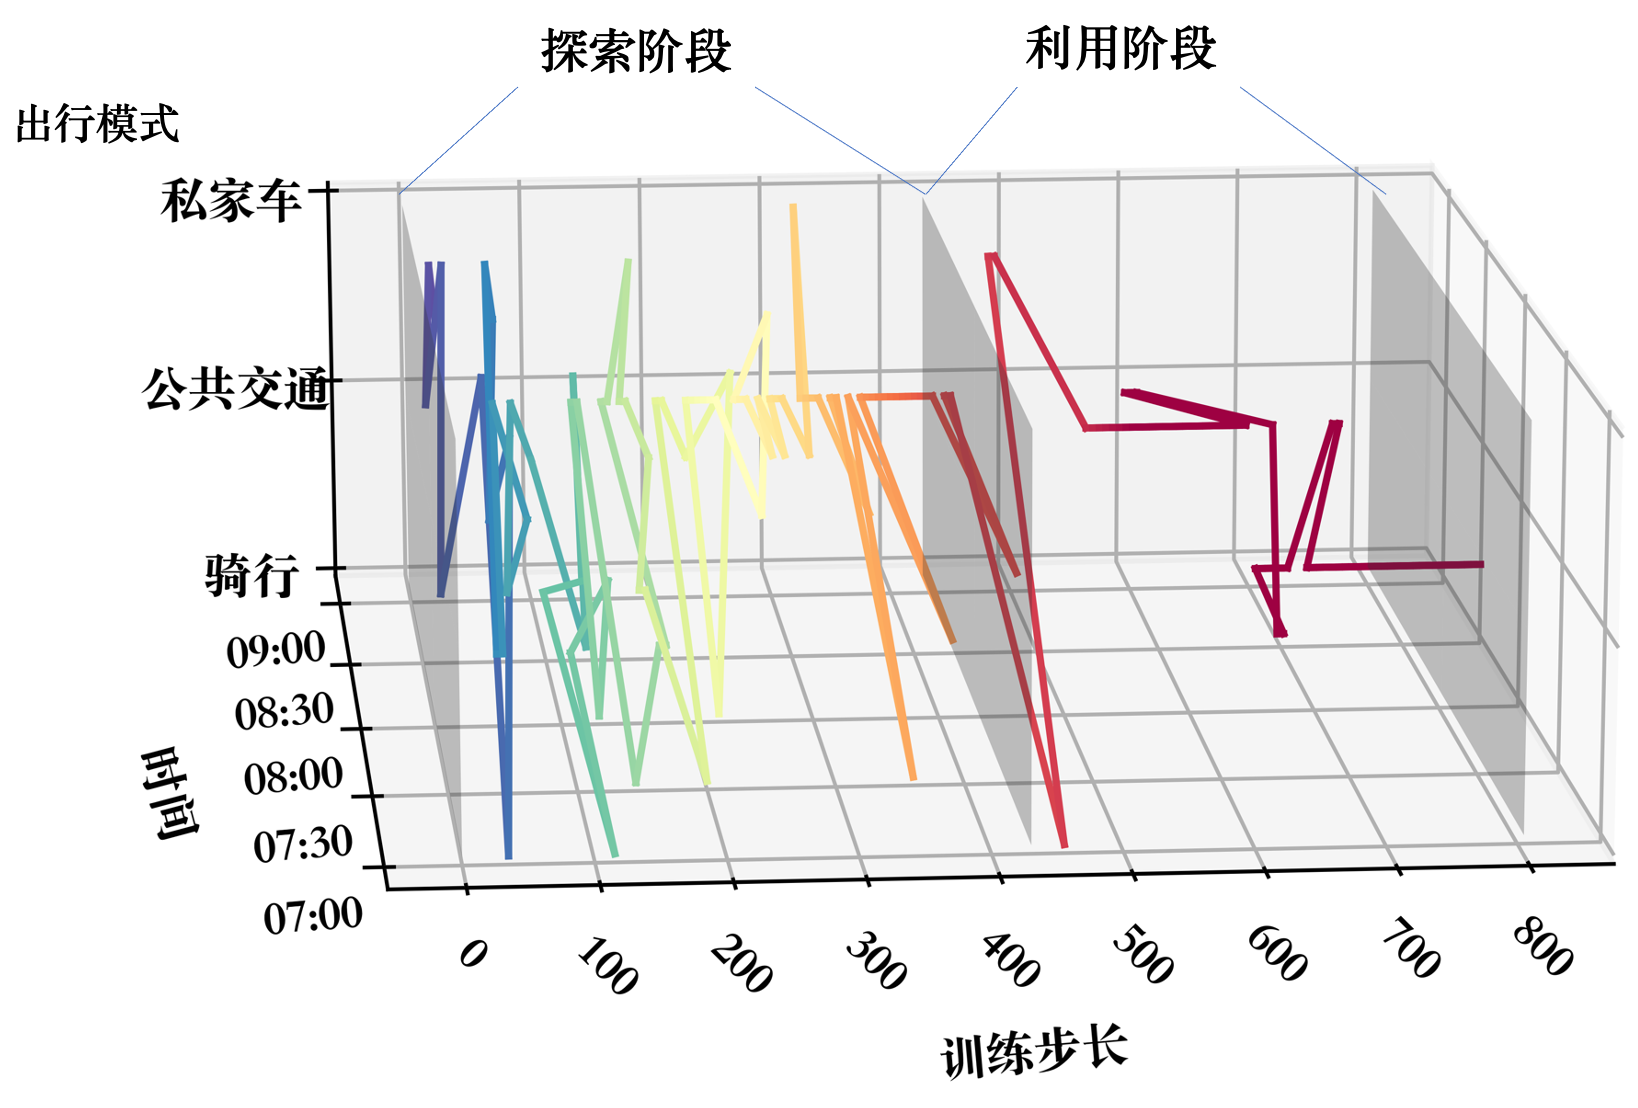
\includegraphics[width=.5\textwidth]{figures/content/action2.png}}
  \\
  \subfloat[Representative \#3]{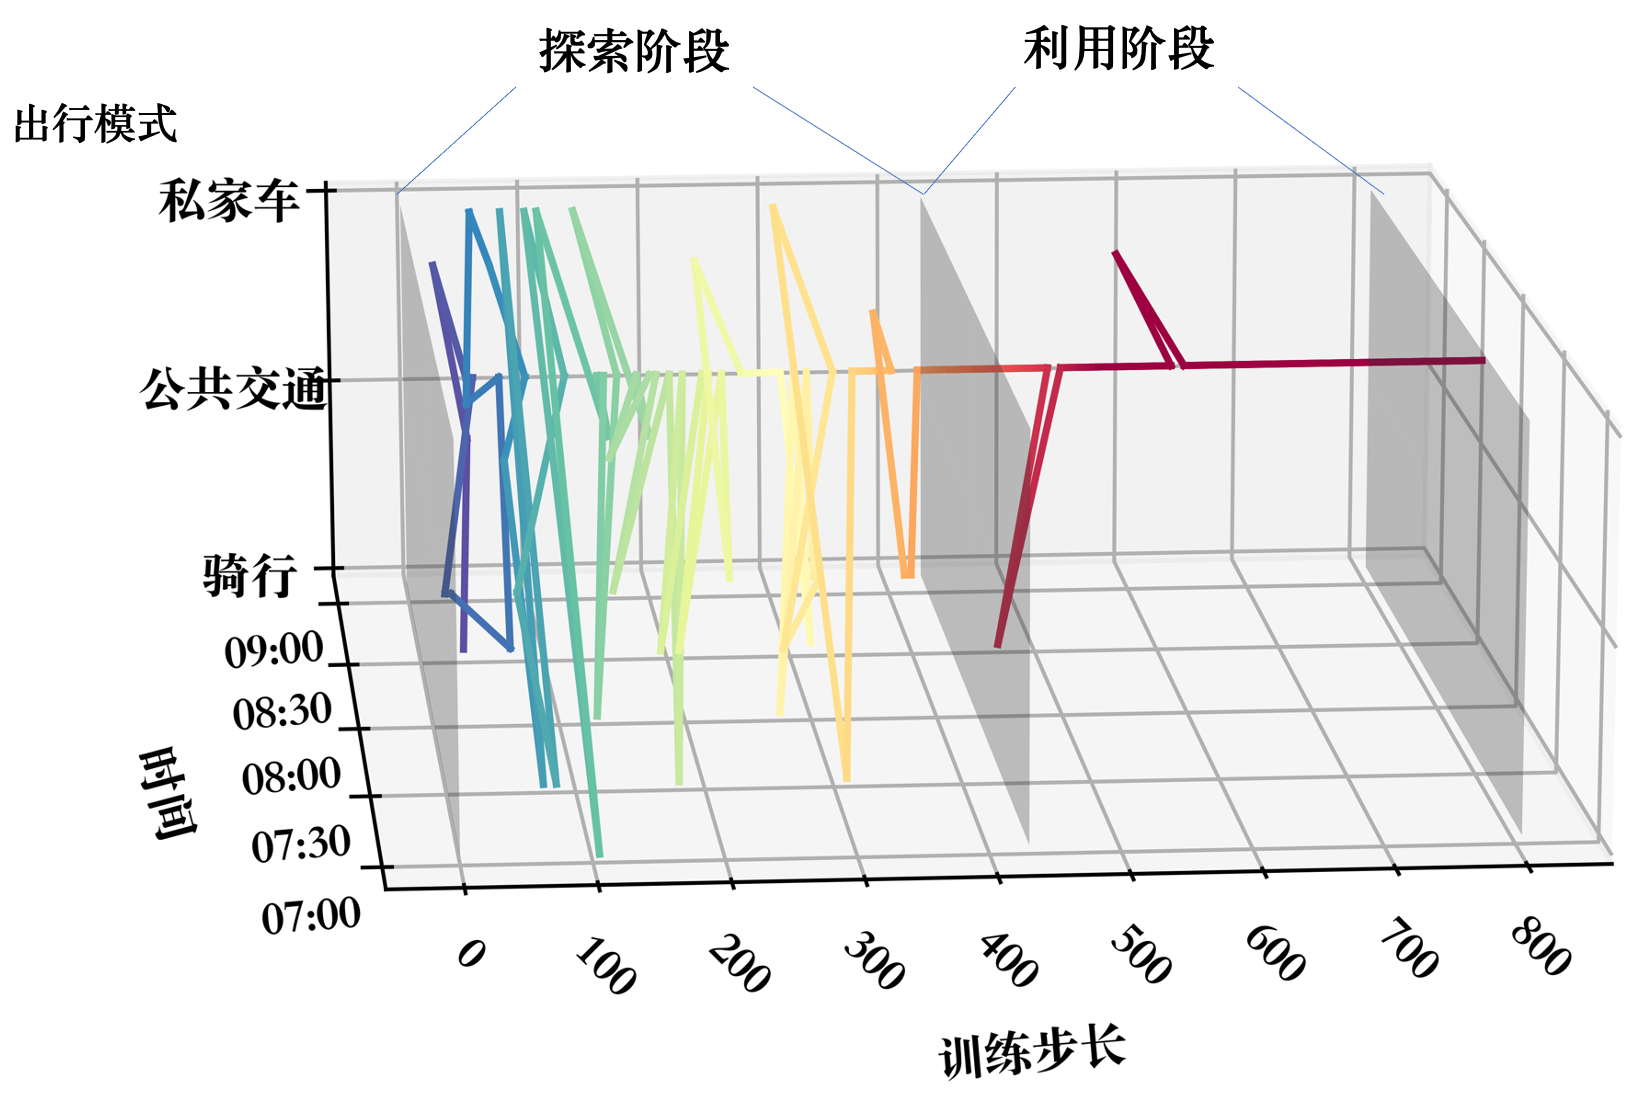
\includegraphics[width=.5\textwidth]{figures/content/action3.png}}
  \quad\quad
  \subfloat[Representative \#4]{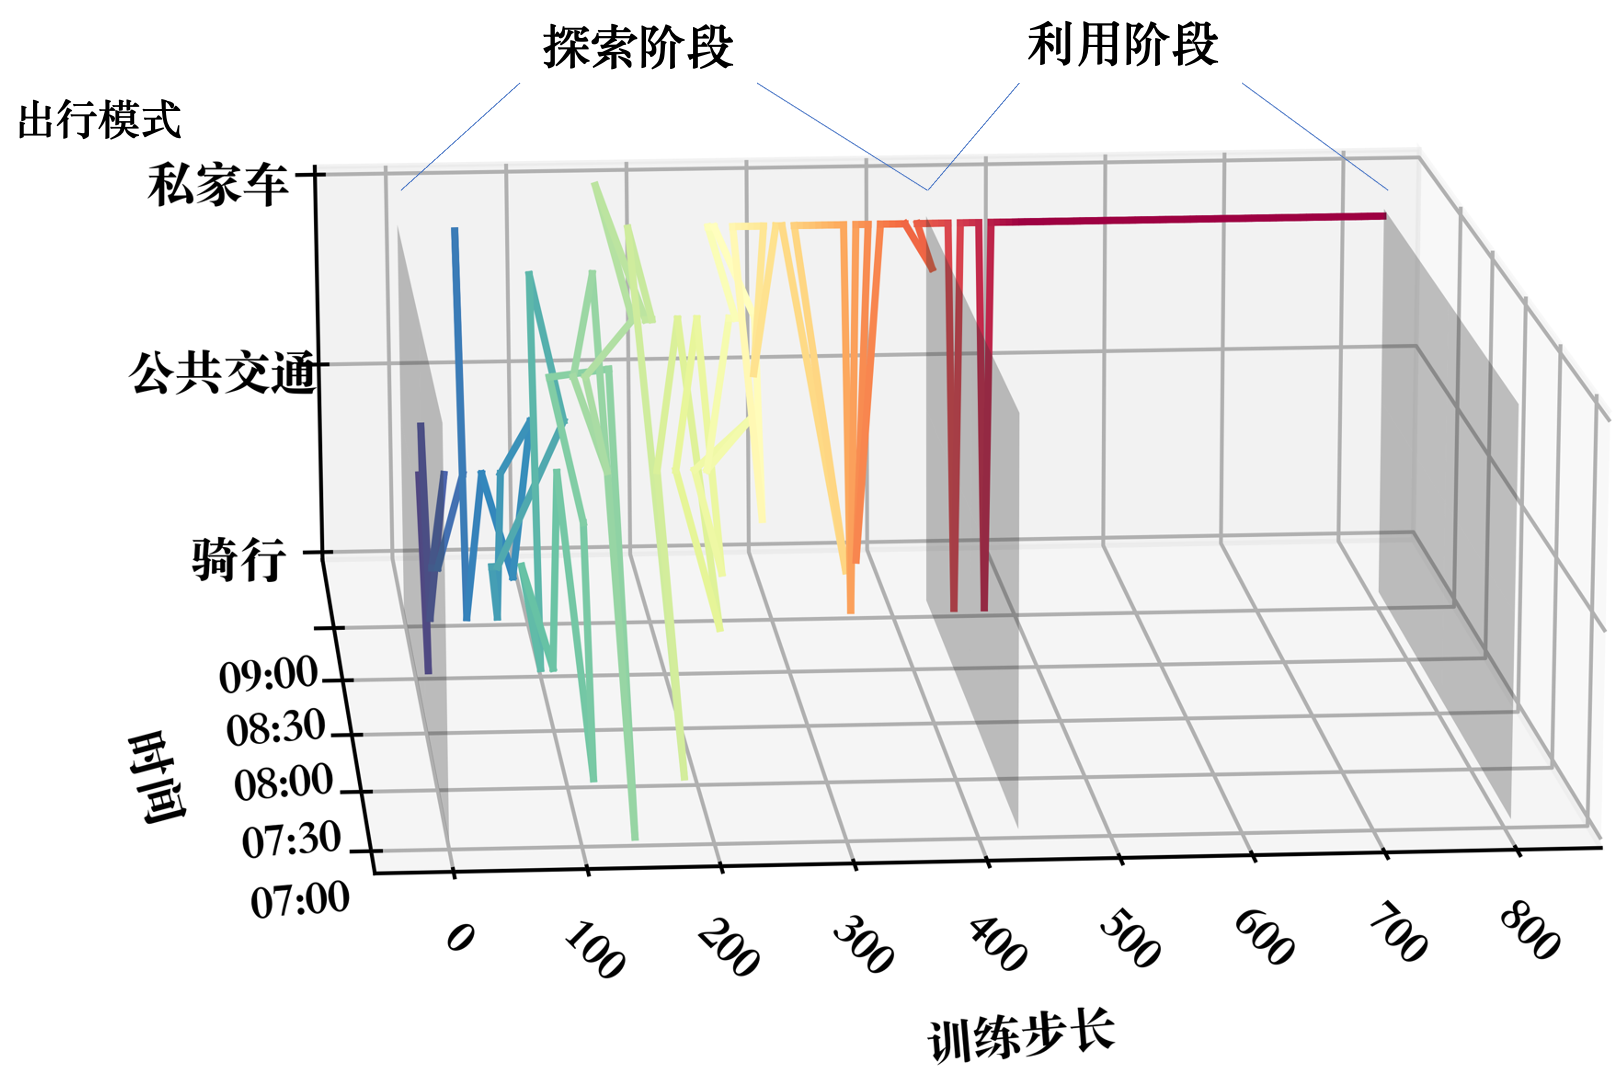
\includegraphics[width=.5\textwidth]{figures/content/action4.png}}
  \caption{Action selections of the four representative individuals.}
  \label{agents}
\end{figure}



通过以上结果,我们证明了所提出的方法是有效的,可以获得JTMDTC问题的良好解决方案。但解决方案的优良程度尚未得到回答。另一个开放的问题涉及训练后的代理程序在其他未参与培训的个体中的适用性或可转移性。接下来将回答这两个问题。

在评估模型的性能时,我们对模型在实际交通流场中的性能进行了测试,并将其与其他常用算法进行了比较。我们选取了四个不同的路口进行测试,并对每个路口的交通情况进行了记录和分析。如图\ref{performance}所示,我们比较了我们的方法和Dijkstra算法以及无DRL的DQN算法(即仅使用简单的Q学习方法)的平均车速。结果表明,相比于其他算法,我们的方法在所有路口的测试中均有更好的表现,表明我们的方法能够有效地提高交通效率。

此外,我们还对模型的泛化能力进行了测试。我们从训练数据中随机选取一部分个体,并将其作为测试集。然后我们对这些测试集中的个体进行测试,并计算其平均奖励值。结果表明,与训练集中的个体相比,测试集中的个体的表现有所下降,但仍然表现出较好的性能,表明我们的模型具有一定的泛化能力。

最后,我们进行了超参数敏感性分析,以确定模型中超参数的最优值。我们分别测试了不同的学习率、批大小和回放缓冲区大小等参数,并记录了模型在测试集上的性能。我们发现,在合理的范围内,这些超参数对模型的性能有较大的影响,因此选择适当的超参数值非常重要。

总的来说,我们的模型表现出了较好的性能和泛化能力,并且具有较强的超参数适应性。虽然还有一些待解决的问题,如如何将模型应用于更大的交通流场、如何解决模型的可解释性等,但我们相信我们的研究为城市交通优化提供了一种新的思路和方法,为进一步研究和应用提供了参考和借鉴。


\section{模型的评估}

为了检验提出方法的优越性或最优性,我们进行了比较分析,将提出的方法与普通的DQN方法以及一种暴力方法进行比较,该方法会随机选择并尝试所有可能的行动。我们选择了50个不参与训练的网络中的测试个体的新的时变OD出行进行比较分析。为了进行比较,我们让每个测试个体根据这些不同决策制定者之一来执行操作,并收集结果奖励。对于暴力方法,执行1,000个周期以完全探索动作空间。

图\ref{com1}、\ref{com2}和\ref{com3}展示了三个选定的测试个体的比较结果。可以看到,暴力方法的奖励显著波动,这是由于随机选择的行动不总是保证良好结果。对于提出的方法和普通的DQN方法,获得的奖励是一个单一值,表示为一条直线,并与JTMDTC问题的最优解相关联。很明显,对于所有三个测试个体,提出的方法给出的解决方案不仅优于普通的DQN方法,而且还优于大多数暴力方法给出的解决方案。事实上,在不聚类个体并利用代表性的情况下,大约有一半的暴力方法给出的解决方案可以击败由普通DQN方法给出的解决方案(见图\ref{com1}和\ref{com2})。

为了从全局角度看待所有50个测试个体的比较,我们找到每个测试个体由暴力方法获得的最大奖励,该奖励被视为JTMDTC问题的(近似)最优解。通过将提出的方法和普通DQN方法给出的解决方案与这个参考值进行比较,我们可以观察到性能差异。如图\ref{com4}所示,提出的方法给出的大多数解决方案(超过50个中的40个)都超过参考值的95%,这意味着这些解决方案接近最优。这对于普通的DQN方法显然不是这样,因为只有约30%的解决方案超过了相同参考值的95%,更不用说还有一些解决方案低于参考值的60%。因此,比较结果表明,在应用于解决具有许多个体的JTMDTC问题时,提出的方法的有效性,以及代表性在完成此任务中发挥的重要作用。由于测试个体不是训练的一部分,因此结果表明提出方法具有很好的可转移性。

\subsection{与传统方法的对比}

现在我们试图考察在信息不完全的情况下,所提出的方法的性能。正如之前所讨论的,部分信息从人类行为学的角度更具相关性,因此预计会导致更差的行动选择。在此,我们还考虑了另外两种模型,用于比较。第一个是一阶马尔可夫链(MC)模型,仅使用当前旅行距离和出发时间差来决定下一个选择。其状态、转移和初始状态概率以及奖励函数均源自DRL模型。两者的主要区别在于决策过程。MC模型使用转移和初始状态概率来模拟随时间变化的行为,而DRL模型使用迭代试错过程。

第二个是传统的MNL模型,使用奖励函数(式(\ref{reward function}))。我们使用在信息完全的情况下,由提出的方法得到的个体出行选择作为基准线,根据其来比较其他模型的性能。考虑了三个性能评估和比较指标。除了奖励之外,另外两个是负对数损失(NLL)和Jaccard指数。这两个指标都衡量其他模型产生的行动与基线获得的行动之间的接近程度或相似程度。因此,它们可以反映其他模型相对于基线的优化水平。但需要注意的是,NLL的较低值是期望的,而对于Jaccard指数,值越高越好。

表\ref{eva}总结了三个性能指标的比较结果。如预期的那样,在信息完全的情况下,所提出的方法提供了实现尽可能多的奖励的最佳性能。所有其他模型的性能都较差,通过比较平均奖励值就能看出这一点,这些值都低于基线的奖励值。这种趋势也适用于NLL和Jaccard指数。尽管如此,在部分信息的情况下,所提出的方法仍然表现出比一阶MC模型和MNL模型略好的性能,这表明即使存在部分信息,所提出的方法仍然是有效的。

\subsection{模型参数的灵敏性分析}

我们现在进行两个敏感性分析,以研究所提出方法在模型参数变化时的性能变化。第一个参数是代表数量,第二个参数是训练个体的集合。为了看到前者的影响,我们进行了进一步的实验,分别使用1、10、20和40个代表。我们保持相同的实验设置,将60个个体的时间依赖OD行程聚类成上述数字,以选择训练代表,而其他50个测试个体则用于评估和比较。同样,蛮力方法作为参考。

比较结果总结在表\ref{cluster_size}中。由于内存溢出,40个代表的实验无法在同一台机器上完成,因此没有报告结果。随着代表数量的增加,所需的训练或计算时间增加,这是预期的。然而,代表数量的增加确实会导致更好的奖励。将一个代表转变为四个代表,奖励得到了最大的提高。进一步将该数字增加到10或20并不能显著提高奖励。这个结果表明,增加代表数量不一定划算。实际上,少量代表已经可以在合理的计算时间内产生相当好的结果。使用蛮力方法得到的最大奖励作为参考值,我们比较了所提出的方法所给出的奖励高于参考值95%以上的测试个体数量。如预期的那样,对于4、10和20个代表,这个数字保持较大且变化很小。图6进一步显示了对于不同数量的代表,四个选定测试个体结果的比较。只有一个代表显然不足以击败蛮力方法,而四个或更多代表则产生了有希望的结果。

为了显示所提出方法的性能并不因训练个体的不同而发生显著变化,我们使用不同的训练个体集合进行另一组实验,使用四个代表对DQN进行训练,其余的实验设置保持不变。表\ref{cluster_agents}总结了这样四个实验的结果。由于不同的训练个体集合不会改变计算时间(对于四个代表,计算时间为22小时),因此不再报告这个度量。从结果中可以看出,所提出方法的性能是稳定的,不会因为用于训练的代表个体不同而表现出显著的变化。类似于图\ref{appendixa1},图\ref{appendixb1}显示了当使用不同的训练个体集合时,四个选定测试个体结果的比较,表明所提出的方法对代表个体的选择具有鲁棒性。这些结果表明,所提出的方法是有效的,不会受到训练代表个体集合的影响。从这些敏感性分析中可以得出结论,所提出的方法在实际应用中具有很强的可操作性和鲁棒性。通过将模型应用于新的时间依赖 OD 数据集并比较与传统模型和暴力方法的性能,我们证明了该方法在解决 JTMDTC 问题方面的有效性。
